%  -*- coding: utf-8 -*-
% !TEX program = xelatex

\documentclass{article}
\usepackage{varwidth}

\usepackage[margin=3.35cm]{geometry}
\usepackage{pgfplots,pgfplotstable}
\pgfplotsset{/pgf/number format/use comma,compat=newest}
\newcommand{\code}[1]{\texttt{#1}}
\usepackage{circuitikz}
\usetikzlibrary{arrows,shapes.gates.logic.US,shapes.gates.logic.IEC,calc}
\usepackage{amsmath}


\begin{document}

\title{Logical/Boolean Arithmetic}
\author{Samuel F. D. Snarksen}
\date{Compiled: \today}
\maketitle

\tableofcontents
\clearpage

\section[Syntax]{Syntax of Boolean expressions}
\subsection{Basic Operators}
There are 2 main operators (the rest can be derived) and 1 modifier. The operators are as the following:

\begin{align}
    \text{And: } & x \cdot y \\
    \text{Or: }  & x + y
\end{align}
\begin{center}
    \text{The only modifier, the negation:} \\
\end{center}
\begin{align}
    \text{Not: } & \bar{x}
\end{align}

\subsection[Derived Operators]{Derived and Advanced Operators}
From our base operators we can now derive some new ones, namely the \code{NAND} (Negated and), \code{NOR} (negated or), \code{XOR} (exclusive or, only one of the inputs can be true, false if they are both true) and \code{XNOR} (negated \code{XOR})\\

The derived operators are quite simple to define (especially the negated operators), they are defined as the following, along with some logical equivalents to some of the base operators: 

\begin{align}
    \text{Nand: } & x \uparrow y \text{ or } \overline{x \cdot y} \\
    \text{Nor: }  & x \downarrow y \text{ or } \overline{x + y}\\
    \text{Xor: }  & x \oplus y \text{ or } (x \cdot \overline{y}) + (\overline{x} \cdot y)\\
    \text{Xnor: } & \overline{x \oplus y} \text{ or } (x \cdot y) + (\overline{x} \cdot \overline{y})
\end{align}
\begin{center}
    Extra definitions for base operators\\
    demonstrated by De Morgan's Law:
\end{center}
\begin{align}
    \text{And: } & \overline{\overline{x} + \overline{y}}\\
    \text{Or: }  & \overline{\overline{x} \cdot \overline{y}}
\end{align}


\section[Adders]{Adders using logic gates}
\subsection{Half-adder}
Below we will construct a table of bits, two in-bits ($IN_1$ and $IN_2$) which will be summed together giving two out-bits ($OUT_1$, $OUT_2$)
which will correspond to the bits of the summed 2-digit long binary number of $IN_1 + IN_2$ (this is the arithmetic `$+$' (plus) operator, not the Boolean `or' operator).

\begin{center}
\begin{tabular}{ | c c | c c | }
 \hline
    $IN_1$ & $IN_2$ & $OUT_1$ & $OUT_2$\\
 \hline
    0 & 0 & 0 & 0\\
 \hline
    0 & 1 & 0 & 1\\
 \hline
    1 & 0 & 0 & 1\\
 \hline
    1 & 1 & 1 & 0\\
 \hline
\end{tabular}
\\ \vspace{2mm} Adder table for two bits to form a new single 2-bit binary number.
\end{center}

One might notice form this table that $OUT_1$ will only be true (1) if both $IN_1$ and $IN_2$ are true (1); we can write this as a Boolean expression: \[OUT_1 = IN_1 \cdot IN_2\]

Now that we have our fist $OUT$, it's time to look at $OUT_2$, one might once again notice that $OUT_2$ is merely the \code{XOR} of $IN_1$ and $IN_2$, written as: \[OUT_2 = IN_1 \oplus IN_2\]

\subsection{Full-adder}
Now that we've constructed a half adder let's create a full-adder giving it three inputs ($IN_1$, $IN_2$ and $IN_3$) it is important to realise that sum of any three 1-digit binary numbers can only result in a 2-digit binary number (think, the max we can sum is $1 + 1 + 1$ which is three, which in binary is $11$)

Let us construct another table:
\begin{center}
\begin{tabular}{ | c c c | c c | }
 \hline
    $IN_1$ & $IN_2$ & $IN_3$ & $OUT_1$ & $OUT_2$\\
 \hline
    0 & 0 & 0 & 0 & 0\\
 \hline
    0 & 0 & 1 & 0 & 1\\
 \hline
    0 & 1 & 0 & 0 & 1\\
 \hline
    0 & 1 & 1 & 1 & 0\\
 \hline
    1 & 0 & 0 & 0 & 1\\
 \hline
    1 & 0 & 1 & 1 & 0\\
 \hline
    1 & 1 & 0 & 1 & 0\\
 \hline
    1 & 1 & 1 & 1 & 1\\
 \hline
\end{tabular}
\\ \vspace{2mm} Adder table for 3 bits to form a new single 2-bit binary number.
\end{center}

This is a full adder, it is called a full adder due to the fact that we're now using all of the outpits available to us, where as before in in the half adder, there was no way to produce, with our 2-bit input, the number three, meaning we weren't using the full potential of our two output bits.\\

The pattern in this table here is a little harder to spot in comparison to the half adder. Let's start with the most obvious, we notice that $OUT_2$ will only be 1, if there are an odd number of bits in $\{IN_1, IN_2, IN_3\}$. This gives us our first clue, using \code{XOR}, since \code{XOR} will only be true if there are an odd number of bits supplied to it. Now how do we make that 

\subsection{Circuit diagrams}
Now let's visualise this by writing it out in the form of logic gates:


\begin{center}
    \tikzstyle{branch}=[fill,shape=circle,minimum size=3pt,inner sep=0pt]
    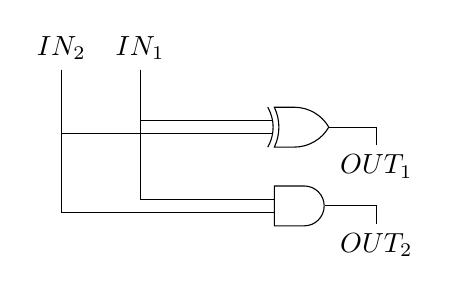
\begin{tikzpicture}[label distance=2mm]
    \node (x1) at (0,0) {$IN_1$};
    \node (x2) at (-1,0) {$IN_2$};
    \node (y1) at (3,-1.5) {$OUT_1$};
    \node (y2) at (3,-2.5) {$OUT_2$};

    \node[xor gate US, draw, logic gate inputs=nn] at ($(2,-1)$)
    (Xor1) {};
    \node[and gate US, draw, logic gate inputs=nn] at ($(2,-2)$)
    (And1) {};
    \draw (x1) |- (Xor1.input 1);
    \draw (x2) |- (Xor1.input 2);
    \draw (x1) |- (And1.input 1);
    \draw (x2) |- (And1.input 2);
    \draw (y2) |- (And1.output);
    \draw (y1) |- (Xor1.output);
    \end{tikzpicture}
\end{center}
Any 

\end{document}